\documentclass[12pt,a4j,twoside]{jarticle}

\usepackage{gradthesis}
\usepackage{amsmath}
\usepackage[dvipdfmx]{graphicx}
\usepackage{amssymb}

\newcommand{\argmax}{\mathop{\rm arg~max}\limits}
\newcommand{\argmin}{\mathop{\rm arg~min}\limits}

\title{未定}{5}
\etitle{hoge}
\author{松本~航平}
\studentid{1W193102}
\university{早稲田大学}
\faculty{基幹理工学部}
\department{情報理工学科}
\type{卒業論文}
\nendo{2022}
\hizuke{2022/}
\advisor{菅原~俊治}

\begin{document}
\maketitle

\begin{abstract}
  本研究では,
\end{abstract}

\vspace*{1cm}\par
\section{研究背景}
近年,ロボット技術が発達し,様々な分野で活躍するようになった.
それに伴い,

\section{関連研究}

\section{モデルの定義}
本研究は\cite{Wu2019}の手法を拡張し,充電基地での待機時間を動的に決定することにより,エネルギー効率の向上を図る.
そこで,従来手法の比較を行うため,本研究に用いるモデルは\cite{Wu2019}と同一のものとする.
この章では,\cite{Wu2019}で用いたモデルについて詳しく説明する.

\subsection{環境}
エージェントの巡回環境を2事変ベクトル空間に埋め込み可能なグラフ$G = (V, E)$で表す.
ここで,$V = \{ v_1, \dots ,v_n \}$はノード集合を表し,各ノード上にエージェントやイベント,障害物が存在する.
また,$E$はノード$v_i$と$v_j$間のエッジ$e_{i, j}$の集合である.

\par
本環境では,単純化のために,エッジの長さはすべて1とする.
$v_i$と$v_j$間の最短距離を$d(v_i, v_j)$,ユークリッド距離を$m(v_i, v_j)$とする.
時間は離散時間であり,その最小単位としてステップを用いる.
各エージェントは,毎ステップ,隣接した障害物のないノードに移動し,そのノード上のイベントを処理することができる.

\par
すべてのノード$v \in V$において,$v$上のイベント発生確率を$p(v) (0 \leq p(v) \leq 1)$とする.
毎時刻$t$において,ノード$v$のイベント発生量$L_t(v)$は,以下の式で更新される.
\begin{equation}
  L_t(v) = 
  \begin{cases}
    L_{t-1}(v) + 1 & \textrm{(イベント発生時)} \\
    L_{t-1}(v)     & \textrm{(その他)}
  \end{cases}
\end{equation}
任意のエージェントが時刻$t$において$v$を訪問と,$v$上のイベントが処理されるため,$L_t(v)$の値は0となる.

\subsection{エージェント}
エージェントの集合を$A=\{1, \dots ,n\}$と表す.
本研究では,各エージェントは自身と他のエージェントの位置が把握できるものとする.
これは,赤外線などのセンサーやGPSを利用することによって実用可能であり,それぞれのエージェントが持つ情報の交換に比べて比較的容易に取得できるためである.
しかし,エージェントの目的地や経路に関する情報は共有しない.
また,単純化のため,同一のノードに複数のエージェントが存在できるものとし,エージェント同士の衝突は考慮しない.

\par
エージェント$i$は,すべてのノード$v$に対し,$v$のイベント発生確率の予測値を表す重要度$p^i(v) (0 \leq p^i(v) \leq 1)$を持つ.
$p^i(v)$は各エージェントが独立して保持しており,その値はエージェントごとに異なる.
各エージェントはこの値を用いてイベント発生量の推定や目標ノードを決定する.

\par
各エージェントはイベント発生量$L(v)$の値を直接把握することはできない.
そのため,エージェント$i$は$p^i(v)$の値を用いて,毎時刻$t$において,ノード$v$のイベント発生量の推定値$EL_t(v)$を以下の式で計算する.
\begin{equation}
  EL^i_t(v) = p^i(v) \times (t - t^v_{vis})
\end{equation}
ここで,$t^v_{vis}$はノード$v$に任意のエージェントが最後に訪問した時刻である.
各エージェントは他のエージェントの位置が把握できるという仮定より,時刻$t^v_{vis}$が分かる.

\par
各エージェントは,十分な容量のバッテリを持ち,充電基地で充電を行う.
エージェント$i$は充電基地$v_{base}$を出発点とし,バッテリを消費しながら環境内を巡回し,再び$v_{base}$に戻り充電をするというサイクルを繰り返す.
エージェント$i$のバッテリ性能を$(B^i_{max}, B^i_{drain}, k^i_{charge})$で表す.
ここで,$B^i_{max}$はエージェントのバッテリ容量,$B^i_{drain}$は1ステップで消費するバッテリ消費量,$k^i_{charge}$はバッテリ残量を1増加させるために必要なステップ数である.
時刻$t$におけるエージェント$i$のバッテリ残量を$b^i(t) (0 \leq b^i(t) \leq B_{max})$とすると,$i$が1ステップで隣接するノードに移動したとき,$b^i(t)$は以下の式に従って更新される.
\begin{equation}
  b^i(t+1) \gets b^i(t) - B^i_{drain}
\end{equation}

\par
$b^i(t)$が0になるとそのエージェントは移動できなくなってしまうので,自身のバッテリ残量が0になる前に戻らなければならない.
そこで,以下の式に示すように,エージェント$i$はノード$v$から充電基地$v_{base}$までの移動に必要な最小バッテリ量であるポテンシャル$\mathcal{P}^i(v)$を計算する.
\begin{equation}
  \mathcal{P}^i(v) = d(v, v_{base}) \times B^i_{drain}
\end{equation}
エージェント$i$は目標ノード$v^i_{tar}$を後の章で説明する目標決定戦略によって決定した際,実際に移動する前に,現在のバッテリ残量で$v^i_{tar}$に到達し,その後充電基地に戻ることができるかを,以下の式を用いて判定する.
\begin{equation}
  b^i(t) \leq \mathcal{P}^i(v) + d(v^i_t, v^i_{tar}) \times B^i_{drain}
\end{equation}
この条件を満たさない場合,以下のように目標ノード$v^i_{tar}$を更新し,充電基地に戻る.
\begin{equation}
  v^i_{tar} \gets v_{base}
\end{equation}
エージェントは充電基地に到着した後,バッテリ残量が最大になるまで充電し,充電が完了した後,再び環境内を巡回する.

\subsection{評価指標}
評価指標は,扱うMACPPの種類によって異なるが,本研究では評価指標としてイベント残存時間の総和$D_{t_s,t_e}$と,エージェントの総エネルギー消費量$C_{t_s,t_e}$を用いる.

\par
本研究のように,MACPPにおける清掃問題の場合,イベントはごみであり,環境内のごみの総量と放置されている時間を減らすことが目的となる.
これを示す指標として,時刻$t_s$から時刻$t_e$までのイベント残存時間の総和$D_{t_s,t_e}$を以下の式で定める.$(t_s < t_e)$
\begin{equation}
  D_{t_s,t_e} = \sum_{v \in V} \sum^{t_e}_{t=t_s+1} L_t(v)
\end{equation}

\par
また,エージェントの総エネルギー消費量を示す指標として,時刻$t_s$から時刻$t_e$までのエネルギー消費量の総和$C_{t_s,t_e}$を以下の式で定める.$(t_s < t_e)$
\begin{equation}
  C_{t_s,t_e} = \sum_{i \in A} \sum^{t_e}_{t=t_s+1} E_t(i)
\end{equation}

\par
一般に,$D_{t_s,t_e}$と$C_{t_s,t_e}$の値はどちらも小さい方が良いとされるが,両者はトレードオフの関係である.
つまり,$D_{t_s,t_e}$と$C_{t_s,t_e}$の値をどちらも最小にすることは困難である.
したがって,\cite{Wu2019}と同様に1stepにおけるイベント量の要求値$D_{req}$を設定した.
ここで,本研究では清掃問題を扱っているため,$D_{t_s,t_e}$が$D_{req}$付近にして,$C_{t_s,t_e}$をより小さくすることを目指す.
また,本研究では単純化のため,これ以降,$D_{t_s,t_e},C_{t_s,t_e}$を$D(s),C(s)$と表す.


\section{準備}
この章では,提案手法の基になったAMTDS ,AMTDS/LD, AMTDS/ESCについて説明する.
これらの手法では,エージェントは目標ノード$v^i_{tar}$を決定する目標決定戦略と,それまでの経路を生成する経路生成戦略に従い,環境内を巡回する.
$v^i_{tar}$に到着した後,再び目標戦略に従って新しい目標ノードを決定するといったサイクルを各エージェントが繰り返し,継続的な環境巡回を行う.

\subsection{Adaptive meta target decision strategy (AMTDS)}
\label{subsec:AMTDS}
この節では,AMTDS/LD, AMTDS/ESCなどの手法のベースとなったAdaptive meta target decision strategy (AMTDS) \cite{Yoneda2013}について説明する.
AMTDSは単純な複数の目標決定戦略の中から,強化学習アルゴリズムであるQ学習によって,各エージェントが自身にとって最適な戦略を選択するメタ戦略学習である.
また,この手法では環境内のすべてのノード$v$におけるイベント発生確率$p(v)$は既知であるという仮定を導入しており,$p^i(v) = p(v)$とする.

\par
エージェント$i$はAMTDSによって目標決定戦略$s \in S$を選択し,$s$に従って目標ノード$v^i_{tar}$を決定する.
その後,経路生成戦略に従って$v^i_{tar}$に移動する.
ここで,$S$はエージェントが選択可能な目標決定戦略の集合である.
目標決定戦略については\ref{target_strategy},経路生成戦略については\ref{route_strategy}で詳細を説明する.
$v^i_{tar}$に到着後,$v^i_{tar}$の決定時刻$t_0$から$d_{travel}$ステップ後に$v^i_{tar}$に到着するまでの1ステップあたりのイベント処理量を以下の式で計算する.
\begin{equation}
  \label{eq:reward_AMTDS}
  u_{t_0,t_0+d_{travel}} = \dfrac{\displaystyle\sum_{t_0+1 \leq t \leq t_0+d_{travel}} L_t(v^i_t)}{d_{travel}}
\end{equation}
さらに,これを報酬として,選択した戦略$s$のQ値$Q^i(s)$を以下の式に従って更新する.
\begin{equation}
  Q^i(s) \gets (1-\alpha)Q^i(s) + \alpha \times u_{t_0,t_0+d_{travel}}
\end{equation}
ここで,$\alpha (0 < \alpha \leq 1)$は学習率である.
$Q^i(s)$の更新後,$i$は次に選択する目標決定戦略$s_{next}$を$\varepsilon$-Greedy法によって決定する.
$\varepsilon$-Greedy法では,$s_{next}$を確率$\varepsilon$でランダムに選択し,確率$1 - \varepsilon$で以下の式に従って選択する.
\begin{equation}
  s_{next} \gets \argmax_{s} Q^i(s)
\end{equation}

\subsubsection{目標決定戦略}
\label{target_strategy}
\cite{Yoneda2013}では,各エージェントに以下の4つの基本的な目標決定戦略を$S$として与えている.
それぞれの戦略は単独でも使用可能な独立したものとなっている.
単独での使用を想定し,競合回避のためにランダム性を取り入れたものも存在する.

\begin{description}
  \item[Random selection (R)]\mbox{}\\
  環境全体のノード集合$V$からランダムに$v^i_{tar}$を選ぶ.

  \item[Probabilistic greedy selection (PGS)]\mbox{} \\
  環境全体のノード集合$V$内のノード$v$におけるイベント発生量の推定値$EL^i_t(v)$の上位$N_g$個のノードから,ランダムに1つ$v^i_{tar}$を選ぶ.
  この際に,学習や訪問をする$v^i_{tar}$の偏りを防ぐため,$N_g$番目のノードと$EL^i_t(v)$の値が同じノードが存在する場合,
  そのノードをすべて含めた後,その中から$v^i_{tar}$をランダムに選んでいる.

  \item[Prioritizing unvisited interval (PI)]\mbox{} \\
  環境全体のノード集合$V$内のノード$v$における訪問間隔$I^i_t(v)$の上位$N_i$個のノードから,ランダムに1つ$v^i_{tar}$を選ぶ.
  この際に,学習や訪問をする$v^i_{tar}$の偏りを防ぐため,$N_i$番目のノードと$I^i_t(v)$の値が同じノードが存在する場合,
  そのノードをすべて含めた後,その中から$v^i_{tar}$をランダムに選んでいる.
  
  \item[Balanced neighbor-preferential selection (BNPS)]\mbox{} \\
  近隣のノードにイベント発生量が多いとエージェントが判断したとき,近隣を優先的に巡回する.
  $v^i_{tar}$の決定時にエージェントの現在地$v^i_t$との距離が$d_{rad}$以下のノード集合を近領域$V^i_{area}$とする.
  ここで,$V^i_{area}$における1ステップあたりのイベント処理量の期待値$EV^i_t$は以下の式で求められる.
  \begin{equation}
    EV^i_t = \frac{\displaystyle \sum_{v \in V^i_{area}}EL^i_t(v)}{|V^i_{area}|}  
  \end{equation}
  エージェント$i$は近領域内のイベントを処理するか判断するための閾値$EV_{threshold}$と$EV^i_t$の値を比較し,
  $EV^i_t > EV_{threshold}$の間はPGSによって近領域内から$v^i_{tar}$を選ぶ.
  その後,$EV^i_t \le EV_{threshold}$となった場合,環境全体を対象とし,PGSで$v^i_{tar}$を選ぶ.
  環境全体から$v^i_{tar}$を選択した後,$V^i_{area}$を更新する.
  更新後の$V^i_{area}$の1ステップあたりのイベント処理量の期待値を$EV^i_{t+1}$とし,$EV_{threshold}$の値を以下の式に従って更新する.
  \begin{equation}
    EV_{threshold} \gets EV_{threshold} + \alpha(EV^i_{t+1} - EV_{threshold})
  \end{equation}
  ここで,$\alpha(0 < \alpha < 1)$は学習率である.また,$EV_{threshold}$の初期値は初めに$V^i_{area}$を設定した際の$EV^i_t$の値である.
\end{description}

\subsubsection{経路生成戦略}
  \label{route_strategy}
  経路生成戦略は{\em gradual path generation} (GPG)を用いる.
  GPGでは,まず$v^i_{tar}$までの最短経路をダイクストラ法を用いて生成し,その経路近辺でイベントが発生しやすいノードを経由するように経路を変更する.
  これにより,最短経路に従うよりも効率を高めることができる.しかし,経由するノードの増加によって$v^i_{tar}$への到着時間が遅れてしまい,逆に効率が下がってしまう.
  そのため,経由するノードに一定の制約をかけなければならない.
  そこで,GPGでは経由可能なノード$v$を以下の式を満たすものとする.
  \begin{equation}
    \begin{cases}
      d(v^i_t, v) \leq d_{myopia} \\
      d(v, v^i_{tar}) < k_{att}(d(v^i_t, v^i_{tar})) \\
      d(v^i_t, v) + d(v, v^i_{tar}) \leq k_{rover}d(v^i_t, v^i_{tar}) \\
      \mathcal{P}^i(v^i_{tar}) + B^i_{drain} \times (d(v^i_t, v) + d(v, v^i_{tar})) \leq b^i(t)
    \end{cases}
  \end{equation}
  ここで,$d_{myopia}$はエージェントが現在地とするノードから経由地点とできるノードまでの距離の閾値であり,$k_{att} (0 < k_{att} < 1)$は$v^i_{tar}$へ引き付ける力を表す係数である.
  また,$k_{rover} (1 < k_{rover})$は経由地点を追加した新しい経路の距離の,最短距離からの増加率である.
  これらの条件を満たすノード集合を$V^i_{sub}$とすると,経由するノード$v^i_{subgoal}$は以下の式で決められる.
  \begin{equation}
    v^i_{subgoal} \gets \argmax_{v \in V^i_{sub}} EL_t(v)
  \end{equation}

  \subsection{AMTDS with learning of dirt accumulation (AMTDS/LD)}
  AMTDSではエージェントが環境内のすべてのノード$v$においてイベント発生確率$p(v)$をあらかじめ把握しているという仮定を導入した.
  しかし,実際の利用を想定すると,イベント発生確率が既知であることはまれである.
  特に本研究のような清掃問題においては,イベントであるごみの発生確率をエージェントが巡回しながら自ら学習するほうがより実用的である.
  そこで,AMTDSに環境のイベント発生確率の学習を加えたAMTDS with learning of dirt accumulation (AMTDS/LD) \cite{sugiyama2015}が提案された.
  AMTDS/LDでは$p^i(v)$の学習アルゴリズムの提案が行われた.以下でこのアルゴリズムについて説明する.
  
  \par
  まず,1ステップ終わるごとにエージェント$i$はすべてのノードについて,そのノードで最後にイベントが処理された時刻$t^v_{vis}$から現在の時刻$t$までの訪問間隔$I^i_t(v)$を以下の式に従って更新する.
  \begin{equation}
    I^i_t(v) = t - t^v_{vis}
  \end{equation}
  その後,$I^i_t(v)$と現在時刻$t$でエージェント$i$が処理したイベント量$L_t(v)$を用いて,$i$の$v$における重要度$p^i(v)$を以下の式に従って更新する.
  \begin{equation}
    p^i(v) \gets (1 - \beta)p^i(v) + \beta \dfrac{L_t(v)}{I^i_t(v)}
  \end{equation}
  ここで,$\beta(0 < \beta \leq 1)$は学習率である.
  AMTDS/LDでは各エージェントが独立した$p^i(v)$の値を保持しているため,それに伴い,イベント発生量の推定値$EL^i_t(v)$もそれぞれ異なる.
  また,同じノード上であってもそのノードへの訪問頻度によって,エージェントのイベントの発生しやすさの認識が異なる.
  このことによって,エージェント間の通信を用いずに$p^i(v)$を用いた間接的な分業が可能になる.
  それにより,AMTDSと比べて競合を回避し,効率も向上した.

  \subsection{AMTDS for energy saving and cleanliness (AMTDS/ESC)}
  AMTDSやAMTDS/LDでは,イベント残存時間をより小さくすることが求められた.
  しかし,エネルギー消費量も同時に小さくすることができればより有用である.
  つまり,イベント残存時間だけではなく,エネルギー消費を節約することが求められることもある.
  したがって,目標決定戦略を選択するQ学習における報酬の計算方法を式(\ref{eq:reward_AMTDS})から以下の式に変更し,報酬を$r_{t_0,t_0+d_{travel}}$とした,AMTDS for energy saving and cleanliness (AMTDS/ESC) \cite{Wu2019}が提案された.
  \begin{equation}
    r_{t_0,t_0+d_{travel}} = \dfrac{\displaystyle\sum_{t_0+1 \leq t \leq t_0+d_{travel}} L_t(v^i_t)}{d_{travel} \times \displaystyle\sum_{t_0+1 \leq t \leq t_0+d_{travel}} E_t(i)}
  \end{equation}
  これにより,エージェントはより少ないエネルギーでより多くのイベントを処理できる目標決定戦略を決定する.
  なお,目標決定戦略$s_{next}$を$\varepsilon$-Greedy法によって決定するのは,\ref{subsec:AMTDS}と同様である.
  
  \par
  AMTDS/ESCではさらに,エネルギー節約行動として,HomingとPausingの2つの行動が導入されている.
  図\ref{fig:flowchart}はエージェントにおける行動選択のフローチャートである.
  このフローチャートが示すように,2つの条件が満たされた場合,エージェントはエネルギー節約行動を行う.
  
  \begin{figure}
    \centering
    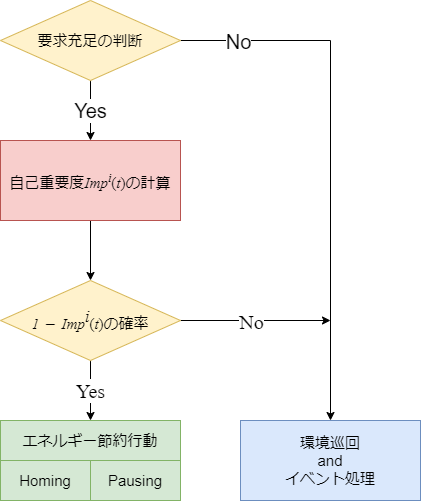
\includegraphics[width=0.6\hsize]{figures/Flowchart.png}
    \caption{エージェントの行動選択}
    \label{fig:flowchart}
  \end{figure}

  \subsubsection{要求充足の判断}
  エージェントは,エネルギー消費を節約すると同時に,総イベント量が与えられた要求値$D_{req}$よりも小さくしなければならないので,次の行動を決定するには,環境全体のイベント量を推定する必要がある.
  そこで,エージェント$i$は自身が持っている$p^i(v)$の値を用いて,以下の式に従って時刻$t$における総イベント量$EV^i_t$を推定する.
  \begin{equation}
    EV^i_t = \sum_{v \in V} EL^i_t(v)
  \end{equation}
  その後,$EV^i_t$が$D_{req}$より小さいかを判断するために,以下の式を用いて,これを満たしていれば$i$は自己重要度評価を行い,満たしていなければ通常通りに環境循環やイベント処理を行う.
  \begin{equation}
    \label{eq:requirement}
    EV^i_t \leq D_{req}
  \end{equation}

  \subsubsection{自己重要度評価}
  式(\ref{eq:requirement})を満たしていたとき,各エージェントは自身がどの程度重要であるかを知るために,エージェントの貢献度を表す自己重要度を評価する.
  エージェントは以下の二つを考慮して,自己の重要度を求める.
  \begin{enumerate}
    \item[(1)] ある期間における過去の貢献度
    \item[(2)] 重要な領域を発見し,その後の行動で多くのイベントを処理できるか
  \end{enumerate}

  \par
  まず,エージェント$i$は,以下の式に従って求められる,短期的な過去の貢献度である$U^i_s$と,長期的な過去の貢献度である$U^i_l$,近い未来における予測される貢献度である$U^i_f$を計算する.
  \begin{equation}
    \begin{cases}
      U^i_s = u_{t_c-T_s, t_c} = \dfrac{\displaystyle \sum_{t_c-T_s < t \leq t_c} EL_t(v^i(t))}{T_s} \\
      U^i_l = u_{t_c-T_l, t_c} = \dfrac{\displaystyle \sum_{t_c-T_l < t \leq t_c} EL_t(v^i(t))}{T_l} \\
      U^i_f = u_{t_c, t_c+T_f} = \dfrac{\displaystyle \sum_{t_c < t \leq t_c+T_f} EL_t(v^i(t))}{T_f}
    \end{cases}
  \end{equation}
  ここで,$t_c$は現在時刻,$T_s$と$T_l$,$T_f$はどのくらいの期間の過去や未来の貢献度を計算するかを決定する固定整数である$(T_s < T_l)$.
  これらを用いて,以下の式に従って自己重要度$Imp^i(t) (0 \leq Imp^i(t) \leq 1)$を求める.
  \begin{equation}
    Imp^i(t) = 
    \begin{cases}
      \dfrac{U^i_s + U^i_f}{U^i_l} & (U^i_s + U^i_f \leq U^i_l) \\
      0                            & (U^i_l = 0) \\
      1                            & (その他)
    \end{cases}
  \end{equation}

  \par
  以上のように求められた$Imp^i(t)$を用いて,以下の式に従って求められた$P^i(t)$の確率で,$i$がHomingやPausingといったエネルギー節約行動を選択する.
  \begin{equation}
    P^i(t) = 1 - Imp^i(t)
  \end{equation}

  \subsubsection{帰還動作 (Homing)}
  この行動は,エージェントが巡回をやめて充電基地に戻ることで,エネルギーを節約する.
  エージェント$i$は$T_{check}$~ステップ移動した後,要求充足の判定や自己重要度評価を行い,Homingを行うかどうかを決定する.
  なお,$i$は電池残量$b^i(t)$が以下の式を満たすときにしか,この行動は行わない.
  \begin{equation}
    b^i(t) < k_{homing} \times B^i_{max} ~~~ (0 < k_{homing} < 1)
  \end{equation}
  この制約は,エージェントが十分に巡回せずに,頻繁に充電基地に戻ることを防ぐために追加している.
  Homingを行うことによって,$i$は$v^i_{tar}$を$v_{base}$に更新し,充電基地に着いたら充電を行う.
  また,Homing中はイベント処理は行うが,要求充足の判定や自己重要度評価は行わない.

  \subsubsection{待機動作 (Pausing)}
  この行動は,エージェントが充電基地で充電が完了した後も,充電基地で待機することで,エネルギーを節約する.
  エージェント$i$は充電基地で充電が完了した後,要求充足の判定や自己重要度評価を行い,Pausingを行うかどうかを決定する.
  Puasing中は,$i$はイベントを処理はせずに,$T_p$~ステップ待機する.

  \section{提案手法}
  AMTDS/ESCにおけるHomingとPausingを組み合わせただけでは,イベント量が要求値$D_{req}$まで許容されていてもエネルギー消費量はほとんど変わらない.
  また,実際に巡回ロボットに適用する場合,イベント量を最小にするよりも,ある程度の要求値$D_{req}$を許容したうえでロボットのバッテリ消費を抑えたほうが,現実的に考えた際に有用である.
  したがって,本研究では充電基地での待機時間を各エージェントが未来の環境全体のイベント量の予測を行い,これを用いて動的に決定する手法をAMTDS/ESCに加えたAMTDS for energy saving under the requirement (AMTDS/ER)と,更にイベント発生量の学習を加えたAMTDS for energy saving under the requirement with learning of event probabilities (AMTDS/ERL)を提案する.

  \subsection{AMTDS for energy saving under the requirement (AMTDS/ER)}
  この節では,AMTDS/ESCをベースに,充電基地での待機時間を各エージェントが動的に決定する手法であるAMTDS/ERについて説明する.

  \subsubsection{HomingとPausingの組み合わせ}
  AMTDS/ESCでは,HomingとPausingはどちらか一方しか実装されていなく,それぞれに対して実験,評価を行った. 
  本研究では,エネルギー消費量をより小さくするために,HomingとPausingを組み合わせ,変更を加えた.
  具体的には,Homingの動作はAMTDS/ESCと同じだが,PausingはAMTDS/ESCのときに加えて,Homingによって充電基地へ帰還し,充電が完了した後は必ずPausingを行うようにした.
  この変更を行った理由は,Homing単体では,エージェントによる,「イベント処理$\rightarrow$充電$\rightarrow$イベント処理$\rightarrow \dotsm$」のサイクルが短くなっただけで,エネルギー消費量に対してはあまり影響がない.
  したがって,Homingを行った後は必ずPausingを行うことによって,エネルギー消費量を小さくすることを目指す.
  
  \subsubsection{補正係数$K$の導入}
  未来のイベント発生量の予測は充電基地での待機中での他のエージェントによるイベント処理を考慮していないため,
  $D_{req}$を超えないように決定した待機時間だけ充電基地で待機しても,実際のイベント残存時間は基本的に$D_{req}$よりも小さくなる.
  従って,エージェントごとに持つ補正係数$K^i$を導入する.これを用いて,イベント残存時間が$D_{req} \times K^i$を超えないように待機時間を決定するようにする.
  また,$K^i$はエージェントが待機し終わって充電基地を出発する際に,実際のイベント量$D_t$を用いて以下の式に従って更新する.
  \begin{equation}
    \begin{cases}
      K^i \gets (1 - \alpha)K^i + \alpha\dfrac{D_{req}}{D_t}K^i & (D_{t} \leq D_{req})\\
      K^i \gets K^i - \left( \dfrac{D_{t}}{D_{req}} - 1 \right) & (D_{t} > D_{req})
    \end{cases}
    \label{eq:K^i}
  \end{equation}

  \subsubsection{未来のイベント発生量の予測}
  エージェントが持っている$p^i(v)$を用いて,$T$step後の未来の環境全体のイベント発生量を以下の式に従って予測する.
  \begin{equation}
    EL^i_{t+T} = \sum_{v \in V} p^i(v) \times \{(t+T)-t^v_{vis}\}
  \end{equation}
  ここで,実行時間の短縮化のため,$T$は$n \times T_{basic} (n \in \mathbb{N})$である.
  本研究では,これを用いて,イベント量$D_t$が$D_{req} \times K^i$を超えないステップまで充電基地で待機するように待機時間を決定する.

  \subsection{AMTDS for energy saving under the requirement with learning of  event probabilities (AMTDS/ERL)}
  AMTDS/ERではエージェントが環境内のすべてのノード$v$においてイベント発生確率$p(v)$をあらかじめ把握しているという仮定を導入した.
  しかし,実際の利用を想定すると,イベント発生確率が既知であることはまれである.
  特に本研究のような清掃問題においては,イベントであるごみの発生確率をエージェントが巡回しながら自ら学習するほうがより実用的である.
  そこで,AMTDS/ERに環境のイベント発生確率の学習を加えたAMTDS/ERLを提案する.AMTDS/ERとの違いは以下の2つである.

  \subsubsection{イベント発生量の予測に使用するノードの範囲の変更}
  AMTDS/ERでは最初からイベント発生確率$p(v)$を把握しているため,環境全体の総イベント発生量の予測の方法は単純である.
  各ノードのイベント発生量を予測し,それを全ノード計算すればよいからである.
  しかし,$p(v)$が未知で学習を行う際には,特に未訪問のノードのイベント発生確率は初期値のままであり,予測が十分に行えない.
  よって,未来のイベント発生量の予測は訪問済みのノード$V_{vis}$のみで行い,その値から訪問済みのノード数$N_{vis}$と壁を除く全ノード数$N_{all}$を用いて以下の式に従って求める.
  なお,学習のためHomingとPausingは$T_{hp}$ ステップまでは行わない.
  \begin{equation}
    EL^i_{t+T} = \sum_{v \in V_{vis}} p^i(v) \times \{ (t+T) - t^v_{vis}\} \times \dfrac{N_{all}}{N_{vis}}
  \end{equation}

  \subsubsection{補正係数$K^i$の更新方法の変更}
  \label{subsec:changeupdate}
  AMTDS/ERでは式(\ref{eq:K^i})に従って$K^i$を更新していたが,AMTDS/ERLでは以下の式に変更した.
  つまり,式(\ref{eq:K^i})の場合分けをなくし,$D_{req}$や$D_t$の値によらず,同じ式で$K^i$を更新するようにした.
  \begin{equation}
    K^i \gets (1 - \alpha)K^i + \alpha\dfrac{D_{req}}{D_t}K^i
  \end{equation}

  \section{評価実験}
  提案手法であるAMTDS/ER,AMTDS/ERLと,従来手法であるAMTDS,AMTDS/LDを比較する実験を行い,D(s)とC(s)を評価指標として用いて,提案手法がイベント量を要求値付近まで許容しつつ,エネルギー消費を抑えることに有効であることを示す.
  加えて,異なる環境においても有効であることも示す.
  最後に,エージェントを途中で停止させ,エージェントのエネルギ抑制行動の変化を分析し,エージェント数の変化によって全体のイベント処理量が変化した際のエージェントの行動の変化を考察する.
  
  \begin{figure}
    \centering
    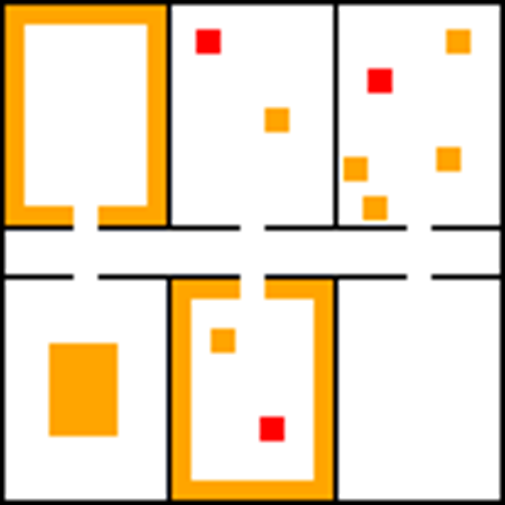
\includegraphics[width=0.6\hsize]{figures/Graph_Office.png}
    \caption{実験環境}
    \label{fig:env}
  \end{figure}

  \subsection{実験環境}
  提案手法の評価実験として,以下に示す実験環境を用意する.
  エージェントが巡回する環境を図で表したものが,図\ref{fig:env}である.
  図\ref{fig:env}に示す通り,環境は6つの部屋で構成されており,部屋と部屋の間には廊下が存在する.
  また,黒色で表した障害物を含む$101 \times 101$の2次元グリッド構造となっている.
  各ノード$v \in V$は座標$(x_v, y_v)~(-50 \leq x_v,y_v \leq 50)$に存在する.
  環境内のノード集合$V$に対して,ノード$v \in V$のイベント発生確率$p(v)$は図\ref{fig:env}の色に応じて,以下の式で表される.
  \begin{equation}
    p(v) = 
    \begin{cases}
      10^{-3}\ & \textrm{(赤色の領域)}\\
      10^{-4}\ & \textrm{(オレンジ色の領域)}\\
      10^{-6}\ & \textrm{(白色の領域)}\\
    \end{cases}
    \label{eq:prob}
  \end{equation}
  色が濃くなるほど,イベントの発生確率が高いことを示す.

  \par
  エージェントの数は20$(|A| = 20)$とし,充電基地$v_{base}$を環境の中心である$(0, 0)$に配置する.
  エージェントはバッテリ残量が最大の状態で$v_{base}$を出発し,自身の戦略で環境内を循環し,バッテリ残量が0になる前に再び$v_{base}$に戻り,充電を行う.
  各エージェントはこの一連の流れを繰り返す.
  すべてのエージェント$i \in A$のバッテリ性能は$(B^i_{max}, B^i_{drain}, k^i_{charge}) = (900, 1, 3)$とする.
  つまり,各エージェントは満充電の状態から最大で900ステップ移動でき,バッテリ残量が0から満充電となるまでに2700ステップかかる.
  したがって,移動と充電のサイクルが最大で3600ステップとなるため,本研究では評価指標$D(s)$と$C(s)$のデータ収集間隔$t_e-t_s$を3600とした.

  \par
  本実験では,1回の試行のステップ数は評価実験によって異なるが,どの評価実験も,試行を50回繰り返した平均値をとる.
  また,本実験で用いるパラメータの値を表\ref{tb:1},表\ref{tb:2},表\ref{tb:3}にまとめた.

  \begin{table}
    \begin{minipage}[t]{.55\textwidth}
      \centering
      \caption{エージェントに関するパラメータ}
      \begin{tabular}{lcr} \\ \hline
        種類 & パラメーター & 値 \\ \hline
        エージェント数 &  |A| & 20 \\ \hline
        バッテリ & $B^i_{max}$ & 900 \\
                   & $B^i_{drain}$ & 1 \\
                   & $k^i_{charge}$ & 3 \\ \hline
        経路生成戦略 & $d_{myopia}$ & 10 \\
                     & $k_{att}$ & 1.0 \\
                     & $k_{rover}$ & 1.2 \\ \hline
      \end{tabular}
      \label{tb:1}
    \end{minipage}
    %
    \hfill
    %
    \begin{minipage}[t]{.55\textwidth}
      \centering
      \caption{目標決定戦略のパラメーター}
      \begin{tabular}{lcrr} \\ \hline
        目標決定戦略 & パラメーター & 値 \\ \hline
        PGS & $N_g$ & 5 \\ \hline
        PI & $N_i$ & 5 \\ \hline
        BNPS & $\alpha$ & 0.1 \\
             & $d_{rad}$ & 15 \\ \hline
        AMTDS & $\alpha$ & 0.1 \\
              & $\varepsilon$ & 0.05 \\ \hline
        AMTDS/LD & $\beta$ & 0.1 \\ \hline 
      \end{tabular}
      \label{tb:2}
    \end{minipage}
    %
    \vskip\baselineskip
    %
    \begin{minipage}[t]{.55\textwidth}
      \centering
      \caption{エネルギー節約行動に関するパラメーター}
      \begin{tabular}{lcrr} \\ \hline
        種類 & パラメーター & 値 \\ \hline
        自己重要度評価 & $T_s$ & 20 \\
                       & $T_l$ & 50 \\
                       & $T_f$ & 10 \\ \hline
        Homing & $T_{check}$ & 100 \\
               & $k_{homing}$ & $\dfrac{1}{3}$ \\ \hline
        Pausing & $T_{basic}$ & 100 \\ \hline  
        AMTDS/ERL & $T_{hp}$ & 500,000 \\ \hline       
      \end{tabular}
      \label{tb:3}
    \end{minipage}
  \end{table}

  \subsection{AMTDS/ERについての実験結果}
  \label{result_ER}
  この節では,提案手法であるAMTDS/ERと,従来手法でありAMTDSにおける評価実験結果を示す.
  複数の条件下での実験結果を,評価指標である$D(s)$と$C(s)$,さらには,必要に応じて他の指標も比較していく.
  

  \begin{figure}
    \centering
    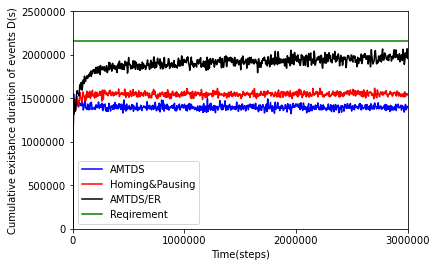
\includegraphics[width=150mm]{figures/ds_graph_3600_ave_ER_Office_600.png}
    \caption{$D(s)$の時間推移の比較(実験1)}
    \label{fig:ds_ER_Office}
  \end{figure}

  \begin{figure}
    \centering
    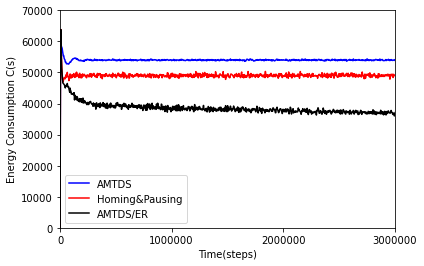
\includegraphics[width=150mm]{figures/cs_graph_3600_ave_ER_Office_600.png}
    \caption{$C(s)$の時間推移の比較(実験1)}
    \label{fig:cs_ER_Office}
  \end{figure}

  \begin{figure}
    \centering
    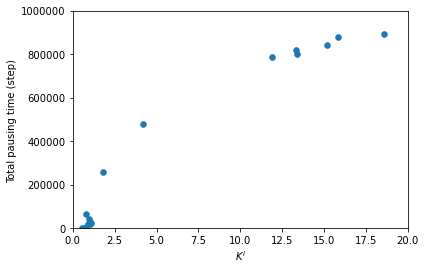
\includegraphics[width=150mm]{figures/CorrectionScatter_Office_ER.png}
    \caption{エージェントごとの$K^i$と総待機時間の関係(実験1)}
    \label{fig:cscatter_ER_Office}
  \end{figure}

  \begin{figure}
    \centering
    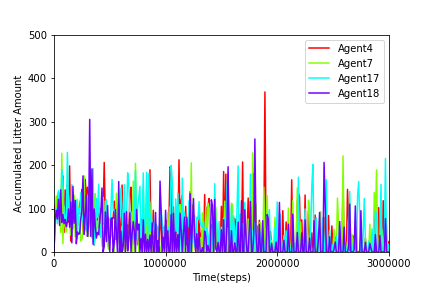
\includegraphics[width=150mm]{figures/al_graph_ER_Office_top.png}
    \caption{$K^i$上位4体のエージェントによるイベント処理量の時間推移(実験1)}
    \label{fig:al_ER_Office_top}
  \end{figure}

  \begin{figure}
    \centering
    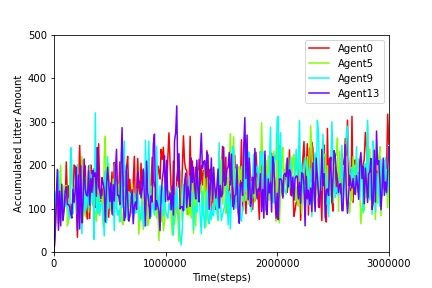
\includegraphics[width=150mm]{figures/al_graph_ER_Office_worst.png}
    \caption{$K^i$下位4体のエージェントによるイベント処理量の時間推移(実験1)}
    \label{fig:al_ER_Office_worst}
  \end{figure}

  \subsubsection{実験1: 性能評価}
  \label{ex:ER1}
  従来手法であるAMTDSと,提案手法であるAMTDS/ERにおける,D(s)とC(s)の比較結果を図\ref{fig:ds_ER_Office},\ref{fig:cs_ER_Office}に示す.
  また,本実験での総ステップ数は3,000,000ステップであり,要求値$D_{req}$は600,補正係数$K^i$の初期値は1.0である.

  \par
  まず,提案手法であるAMTDS/ERは,D(s)の値を従来手法であるAMTDSよりも増加させ,$D_{req}$に近づけられていることが分かる.
  それにより,C(s)の値をAMTDSよりも減少させることができた.
  具体的には,D(s)を$D_{req}$に近づけて約35.5\%増加させることにより,C(s)を約28.2\%削減した.
  つまり,AMTDS/ERのエネルギー節約行動により,環境全体の汚れを$D_{req}$付近にしつつ,より省エネな巡回が行うことができた.
  
  \par
  次に,環境全体ではなく,エージェントごとについて見ていく.
  AMTDS/ERでは,$D(s)$や$C(s)$の変化は補正係数$K^i$によって計算されるPausingによる充電基地での待機時間の影響が大きい.
  また,これらは各エージェントによって異なるため,それに伴ってエージェントの行動も変わってくる.
  エージェントごとの$K^i$とPausingによる総待機時間をまとめたものが表\ref{tb:ER_Office_k1},\ref{tb:ER_Office_k2},\ref{tb:ER_Office_k3}であり,これを散布図にまとめたものが図\ref{fig:cscatter_ER_Office}である.
  なお,$K^i$は3,000,000ステップ時点の値で,総待機時間は2,000,000~3,000,000ステップでの総待機時間である.
  これらの表から,エージェントによって$K^i$は大きく異なり,それによって総待機時間も異なっていることがわかる.
  また,エージェント通しで$K^i$の値や総待機時間といった情報の交換は行われていないが,Pausingを行わずに通常通り環境を巡回するエージェントと,1,000,000ステップの間,充電基地で待機している時間が長いエージェントとの役割分担が自然に行われたということが分かる.
  特に,エージェント1,3,6,8,9は1,000,000ステップのうち,Pausingによる充電基地での待機は行っていないのに対し,エージェント17は810,900ステップも待機している.
  巡回と充電のサイクルが最大で3,600ステップであり,通常はこのサイクルを1,000,000ステップでは少なくとも277回行うが,エージェント17は225.25サイクル分の巡回を行わずに充電基地で待機していたということが分かる.
  
  \par
  さらに,各エージェントのイベント処理量の時間推移のうち,$K^i$が上位4体を図\ref{fig:al_ER_Office_top},下位4体を図\ref{fig:al_ER_Office_worst}に示す.
  まず,図\ref{fig:al_ER_Office_top}より,時間が経つにつれて$K^i$が大きくなったエージェントは,それに伴って充電基地での待機時間が長くなるため,環境を巡回する時間が短くなり,イベント処理量がだんだんと少なくなっていくことが分かる.
  逆に,図\ref{fig:al_ER_Office_worst}より,$K^i$が小さいエージェントはだんだんとイベント処理量が多くなっていることが分かる.
  これは,複数のエージェントの充電基地での待機時間が長くなると,ノード$v$が任意のエージェントに訪問される間隔が長くなり,それによってイベントが溜まっていくので,$K^i$が小さいエージェントのイベント処理量がだんだん多くなっていると考えられる.

  \par
  以上のことから,AMTDS/ERは,AMTDSのように環境全体のイベント発生確率をあらかじめ把握した中で,イベント量を与えられた要求値付近にすることで,エネルギーを節約しながら巡回することができる手法といえる.

  \begin{table}
    \centering
    \caption{エージェント0~6における$K^i$と総待機時間の比較(実験1)}
    \begin{tabular}{lcccccccr}\\ \hline
      エージェント & 0 & 1 & 2 & 3 & 4 & 5 & 6 \\ \hline
      $K^i$ & 11.0250 & 0.5079 & 0.8457 & 0.5082 & 6.0391 & 7.7298 & 0.6987 \\ \hline
      総待機時間 & 786,800 & 0 & 28,100 & 0 & 609,700 & 698,600 & 0 \\ \hline      
    \end{tabular}
    \label{tb:ER_Office_k1}
  \end{table}

  \begin{table}
    \centering
    \caption{エージェント7~13における$K^i$と総待機時間の比較(実験1)}
    \begin{tabular}{lcccccccr}\\ \hline
      エージェント & 7 & 8 & 9 & 10 & 11 & 12 & 13 \\ \hline
      $K^i$  & 0.7758 & 0.5405 & 0.4826 & 0.7002 & 9.5671 & 0.7050 & 0.8753 \\ \hline
      総待機時間 & 144,000 & 0 & 0 & 1,000 & 771,300 & 3,700 & 1,800 \\ \hline      
    \end{tabular}
    \label{tb:ER_Office_k2}
  \end{table}

  \begin{table}
    \centering
    \caption{エージェント14~19における$K^i$と総待機時間の比較(実験1)}
    \begin{tabular}{lccccccr}\\ \hline
      エージェント & 14 & 15 & 16 & 17 & 18 & 19 \\ \hline
      $K^i$  & 9.1121 & 10.1859 & 0.6054 & 11.8902 & 11.6212 & 0.8252 \\ \hline
      総待機時間 & 770,800 & 759,800 & 400 & 810,900 & 798,700 & 12,200 \\ \hline      
    \end{tabular}
    \label{tb:ER_Office_k3}
  \end{table}

  \begin{figure}
    \centering
    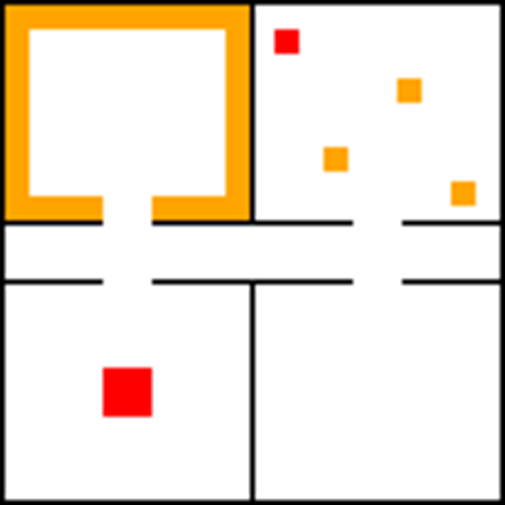
\includegraphics[width=0.6\hsize]{figures/Graph_Complex.png}
    \caption{実験環境(全体のイベント発生確率が小さい場合)}
    \label{fig:env2}
  \end{figure}

  \begin{figure}
    \centering
    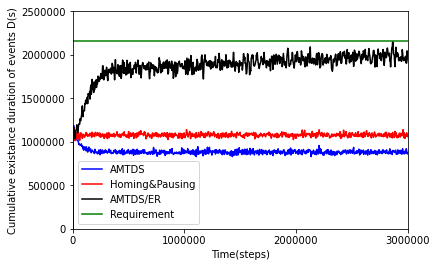
\includegraphics[width=150mm]{figures/ds_graph_3600_ave_ER_Complex_600.png}
    \caption{$D(s)$の時間推移の比較(実験2)}
    \label{fig:ds_ER_Complex}
  \end{figure}

  \begin{figure}
    \centering
    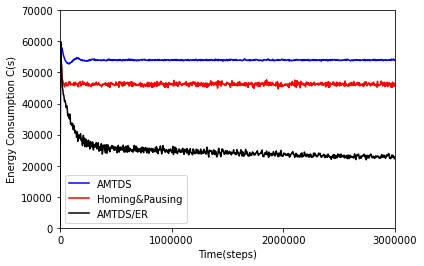
\includegraphics[width=150mm]{figures/cs_graph_3600_ave_ER_Complex_600.png}
    \caption{$C(s)$の時間推移の比較(実験2)}
    \label{fig:cs_ER_Complex}
  \end{figure}

  \begin{figure}
    \centering
    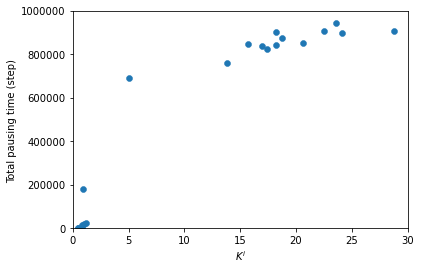
\includegraphics[width=150mm]{figures/CorrectionScatter_Complex_ER.png}
    \caption{エージェントごとの$K^i$と総待機時間の関係(実験2)}
    \label{fig:cscatter_ER_Complex}
  \end{figure}

  \begin{figure}
    \centering
    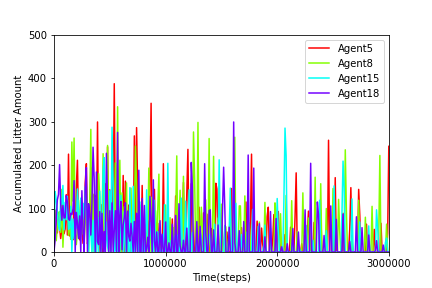
\includegraphics[width=150mm]{figures/al_graph_ER_Complex_top.png}
    \caption{$K^i$上位4体のエージェントによるイベント処理量の時間推移(実験2)}
    \label{fig:al_ER_Complex_top}
  \end{figure}

  \begin{figure}
    \centering
    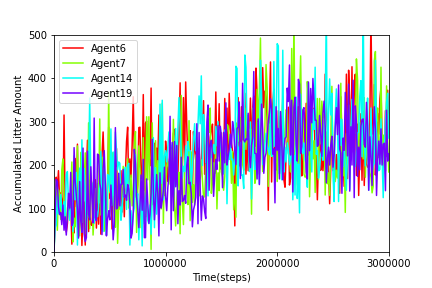
\includegraphics[width=150mm]{figures/al_graph_ER_Complex_worst.png}
    \caption{$K^i$下位4体のエージェントによるイベント処理量の時間推移(実験2)}
    \label{fig:al_ER_Complex_worst}
  \end{figure}

  \subsubsection{実験2: 環境の変化による性能の違い}
  \label{ex:ER2}
  本実験では,図\ref{fig:env}とは異なる環境である,環境全体のイベント発生確率がより小さい環境を新しく用意し,実験を行った.
  その環境を図\ref{fig:env2}に示す.
  ここでは,環境全体のイベント発生量が異なっても,提案手法が有効であるかを検証するため,図の色の濃さに対応するイベント発生確率は式(\ref{eq:prob})と同じであるが,色のついたノードの数を減らしている.
  また,比較を容易にするために,\ref{ex:ER1}と同様に,本実験での総ステップ数は3,000,000ステップであり,要求値$D_{req}$は600,補正係数$K^i$の初期値は1.0である.

  \par
  まず,提案手法であるAMTDS/ERは,異なる環境においても,D(s)の値を従来手法であるAMTDSよりも増加させ,$D_{req}$に近づけ,C(s)の値をAMTDSよりも減少させることができた.
  具体的には,D(s)を$D_{req}$に近づけて約112.5\%増加させることにより,C(s)を約54.1\%削減した.
  つまり,AMTDS/ERのエネルギー節約行動により,環境全体の汚れを$D_{req}$付近にしつつ,より省エネな巡回が行うことができた.
  また,\ref{ex:ER1}と比べると,環境全体のイベント発生量は小さくても要求値$D_{req}$を同じであるので,D(s)の増加率が大きくなるため,それに伴いC(s)の減少率も大きくなった.
  
  \par
  次に,環境全体ではなく,エージェントごとについて見ていく.
  エージェントごとの$K^i$とPausingによる総待機時間をまとめたものが表\ref{tb:ER_Complex_k1},\ref{tb:ER_Complex_k2},\ref{tb:ER_Complex_k3}であり,これを散布図にまとめたものが図\ref{fig:cscatter_ER_Complex}である.
  なお,\ref{ex:ER1}と同様に,$K^i$は3,000,000ステップ時点の値で,総待機時間は2,000,000~3,000,000ステップでの総待機時間である.
  これらの表から,エージェントによって$K^i$は大きく異なり,それによって総待機時間も異なっていることがわかる.
  また,エージェント通しで$K^i$の値や総待機時間といった情報の交換は行われていないが,Pausingを行わずに通常通り環境を巡回するエージェントと,1,000,000ステップの間,充電基地で待機している時間が長いエージェントとの役割分担が自然に行われたということが分かる.
  特に,エージェント17,18,は1,000,000ステップのうち,Pausingによる充電基地での待機は行っていないのに対し,エージェント9は905,600ステップも待機している.
  巡回と充電のサイクルが最大で3,600ステップであり,通常はこのサイクルを1,000,000ステップでは少なくとも277回行うが,エージェント9は約251.6サイクル分の巡回を行わずに充電基地で待機していたということが分かる.
  さらに,図\ref{fig:cscatter_ER_Office}では充電基地に待機している時間が長いエージェントは8体だが,図\ref{fig:cscatter_ER_Complex}では14体に増えている.
  これは,本実験の環境である図\ref{fig:env2}は図\ref{fig:env}と比べて環境全体のイベント発生確率が小さいため,同じ要求値$D_{req}$が与えられると,D(s)要求値付近にするためには,巡回を行わずに充電基地で待機する時間を長くしなければいけないので,待機するエージェントが増加したと考えられる.
  
  \par
  さらに,各エージェントのイベント処理量の時間推移のうち,$K^i$が上位4体を図\ref{fig:al_ER_Complex_top},下位4体を図\ref{fig:al_ER_Complex_worst}に示す.
  まず,図\ref{fig:al_ER_Complex_top}より,時間が経つにつれて$K^i$が大きくなったエージェントは,それに伴って充電基地での待機時間が長くなるため,環境を巡回する時間が短くなり,イベント処理量がだんだんと少なくなっていくことが分かる.
  逆に,図\ref{fig:al_ER_Complex_worst}より,$K^i$が小さいエージェントはだんだんとイベント処理量が多くなっていることが分かる.
  これは,複数のエージェントの充電基地での待機時間が長くなると,ノード$v$が任意のエージェントに訪問される間隔が長くなり,それによってイベントが溜まっていくので,$K^i$が小さいエージェントのイベント処理量がだんだん多くなっていると考えられる.

  \par
  以上のことから,AMTDS/ERは,環境が異なっても,充電基地での待機時間を変化させることによってイベント量を要求値付近にして,エネルギーを節約しながら巡回することができる手法といえる.

  \begin{table}
    \centering
    \caption{エージェント0~6における$K^i$と総待機時間の比較(実験2)}
    \begin{tabular}{lcccccccr}\\ \hline
      エージェント & 0 & 1 & 2 & 3 & 4 & 5 & 6 \\ \hline
      $K^i$ & 14.4864 & 14.2702 & 21.0839 & 14.2977 & 0.6541 & 12.2702 & 11.0955 \\ \hline
      総待機時間 & 843,300 & 846,800 & 877,400 & 840,800 & 4,200 & 808,600 & 861,400 \\ \hline      
    \end{tabular}
    \label{tb:ER_Complex_k1}
  \end{table}

  \begin{table}
    \centering
    \caption{エージェント7~13における$K^i$と総待機時間の比較(実験2)}
    \begin{tabular}{lcccccccr}\\ \hline
      エージェント & 7 & 8 & 9 & 10 & 11 & 12 & 13 \\ \hline
      $K^i$  & 18.9945 & 14.6801 & 21.5276 & 8.5475 & 18.3532 & 19.2192 & 0.5416 \\ \hline
      総待機時間 & 905,500 & 855,200 & 905,600 & 771,000 & 875,400 & 883,600 & 10,400 \\ \hline      
    \end{tabular}
    \label{tb:ER_Complex_k2}
  \end{table}

  \begin{table}
    \centering
    \caption{エージェント14~19における$K^i$と総待機時間の比較(実験2)}
    \begin{tabular}{lccccccr}\\ \hline
      エージェント & 14 & 15 & 16 & 17 & 18 & 19 \\ \hline
      $K^i$  & 0.8083 & 12.1195 & 0.7170 & 0.4826 & 0.3332 & 9.3735 \\ \hline
      総待機時間 & 1,100 & 824,900 & 10,200 & 0 & 0 & 790,600 \\ \hline
    \end{tabular}
    \label{tb:ER_Complex_k3}
  \end{table}

  \subsubsection{実験3: エージェント数減少による性能の変化}

  \subsubsection{実験4: $K^i$の降順にエージェント数を減少させたときの性能の変化}

  \subsection{AMTDS/ERLについての実験結果}
  \label{result_ERL}
  この節では,提案手法であるAMTDS/ERLと,従来手法でありAMTDS/LDにおける評価実験結果を示す.
  節\ref{result_ER}と同様に,複数の条件下での実験結果を,評価指標である$D(s)$と$C(s)$,さらには,必要に応じて他の指標も比較していく.
  なお,AMTDS/ERLはイベント発生確率の学習のため,エネルギー節約行動は500,000ステップから行っている.

  \begin{figure}
    \centering
    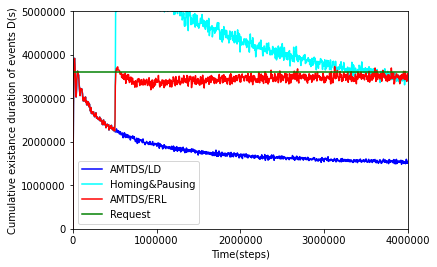
\includegraphics[width=150mm]{figures/ds_graph_3600_ave_ERL_Office_1000.png}
    \caption{$D(s)$の時間推移の比較(実験5)}
    \label{fig:ds_ERL_Office}
  \end{figure}

  \begin{figure}
    \centering
    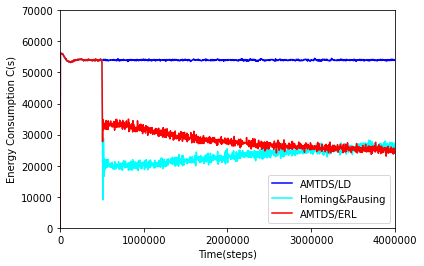
\includegraphics[width=150mm]{figures/cs_graph_3600_ave_ERL_Office_1000.png}
    \caption{$C(s)$の時間推移の比較(実験5)}
    \label{fig:cs_ERL_Office}
  \end{figure}

  \begin{figure}
    \centering
    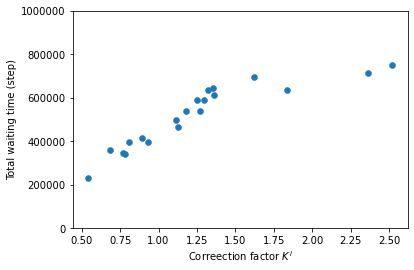
\includegraphics[width=150mm]{figures/CorrectionScatter_Office_ERL.png}
    \caption{エージェントごとの$K^i$と総待機時間の関係(実験5)}
    \label{fig:cscatter_ERL_Office}
  \end{figure}

  \begin{figure}
    \centering
    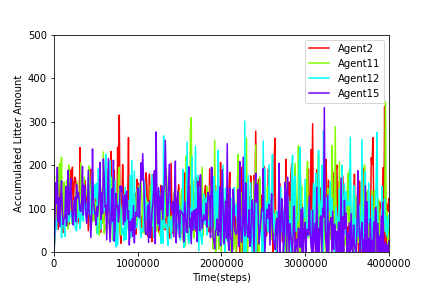
\includegraphics[width=150mm]{figures/al_graph_ERL_Office_top.png}
    \caption{$K^i$上位4体のエージェントによるイベント処理量の時間推移(実験5)}
    \label{fig:al_ERL_Office_top}
  \end{figure}

  \begin{figure}
    \centering
    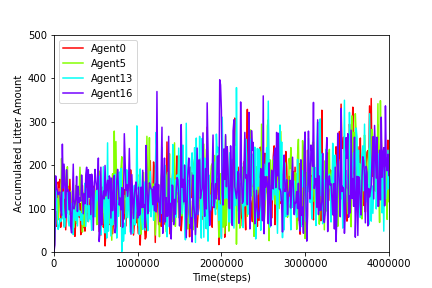
\includegraphics[width=150mm]{figures/al_graph_ERL_Office_worst.png}
    \caption{$K^i$下位4体のエージェントによるイベント処理量の時間推移(実験5)}
    \label{fig:al_ERL_Office_worst}
  \end{figure}

  \subsubsection{実験5: 性能評価}
  \label{ex:ERL1}
  従来手法であるAMTDS/LDと,提案手法であるAMTDS/ERLにおける,D(s)とC(s)の比較結果を図\ref{fig:ds_ERL_Office},\ref{fig:cs_ERL_Office}に示す.
  また,本実験での総ステップ数は4,000,000ステップであり,要求値$D_{req}$は1,000,補正係数$K^i$の初期値は0.5である.

  \par
  まず,提案手法であるAMTDS/ERLは,D(s)の値を従来手法であるAMTDS/LDよりも増加させ,$D_{req}$に近づけられていることが分かる.
  それにより,C(s)の値をAMTDS/LDよりも減少させることができた.
  具体的には,D(s)を$D_{req}$に近づけて約82.4\%増加させることにより,C(s)を約42.2\%削減した.
  また,図\ref{fig:ds_ER_Office}と比較すると,AMTDS/ERLの方が要求値により近づけられている.
  これは,\ref{subsec:changeupdate}で$K^i$の更新方法を変更したためである.
  つまり,AMTDS/ERLのエネルギー節約行動により,環境全体の汚れを$D_{req}$付近にしつつ,より省エネな巡回が行うことができた.
  
  \par
  次に,環境全体ではなく,エージェントごとについて見ていく.
  AMTDS/ERLもAMTDS/ERと同様に,$D(s)$や$C(s)$の変化は補正係数$K^i$によって計算されるPausingによる充電基地での待機時間の影響が大きい.
  また,これらは各エージェントによって異なるため,それに伴ってエージェントの行動も変わってくる.
  エージェントごとの$K^i$とPausingによる総待機時間をまとめたものが表\ref{tb:ERL_Office_k1},\ref{tb:ERL_Office_k2},\ref{tb:ERL_Office_k3}であり,これを散布図にまとめたものが図\ref{fig:cscatter_ERL_Office}である.
  なお,$K^i$は4,000,000ステップ時点の値で,総待機時間は3,000,000~4,000,000ステップでの総待機時間である.
  これらの表から,エージェントによって$K^i$は異なり,それによって総待機時間も異なっていて,基本的に充電基地で待機しているエージェントと,あまり待機しないエージェントが存在していることがわかる.
  しかし,図\ref{fig:cscatter_ER_Office}と比較すると,$K^i$にしっかりとしたグループ分けのようなものは存在していない.
  これも,\ref{subsec:changeupdate}での$K^i$の更新方法を変更したためであると考えられる.
  また,AMTSD/ERはあらかじめノード$v$におけるイベント発生確率$p(v)$が与えられ,これが変更されることはないが,AMTDS/ERLは$p^i(v)$の学習を行っているので,巡回するたびに環境全体のイベント発生確率の予測値が変化するということも影響していると考えられる.
  
  \par
  さらに,各エージェントのイベント処理量の時間推移のうち,$K^i$が上位4体を図\ref{fig:al_ERL_Office_top},下位4体を図\ref{fig:al_ERL_Office_worst}に示す.
  まず,図\ref{fig:al_ERL_Office_top}より,時間が経つにつれて$K^i$が大きくなったエージェントは,それに伴って充電基地での待機時間が長くなるため,環境を巡回する時間が短くなり,イベント処理量がだんだんと少なくなっていくことが分かる.
  逆に,図\ref{fig:al_ERL_Office_worst}より,$K^i$が小さいエージェントはだんだんとイベント処理量が多くなっていることが分かる.
  これは,複数のエージェントの充電基地での待機時間が長くなると,ノード$v$が任意のエージェントに訪問される間隔が長くなり,それによってイベントが溜まっていくので,$K^i$が小さいエージェントのイベント処理量がだんだん多くなっていると考えられる.

  \par
  以上のことから,AMTDS/ERLはAMTDS/LDのように,各ノードのイベント発生確率を学習しながら巡回し,イベント量を与えられた要求値付近にすることで,エネルギーを節約しながら巡回することができる手法といえる.

  \begin{table}
    \centering
    \caption{エージェント0~6における$K^i$と総待機時間の比較(実験5)}
    \begin{tabular}{lcccccccr}\\ \hline
      エージェント & 0 & 1 & 2 & 3 & 4 & 5 & 6 \\ \hline
      $K^i$ & 0.5414 & 1.2494 & 1.3542 & 1.1793 & 1.2972 & 0.7833 & 2.3616 \\ \hline
      総待機時間 & 228,000 & 586,400 & 643,800 & 538,500 & 587,700 & 339,800 & 712,300 & \\ \hline      
    \end{tabular}
    \label{tb:ERL_Office_k1}
  \end{table}

  \begin{table}
    \centering
    \caption{エージェント7~13における$K^i$と総待機時間の比較(実験5)}
    \begin{tabular}{lcccccccr}\\ \hline
      エージェント & 7 & 8 & 9 & 10 & 11 & 12 & 13 \\ \hline
      $K^i$  & 0.8060 & 0.8948 & 1.8351 & 0.9304 & 1.6217 & 1.3595 & 0.7680 \\ \hline
      総待機時間 & 393,900 & 416,100 & 636,500 & 395,500 & 696,500 & 611,600 & 343,800 \\ \hline      
    \end{tabular}
    \label{tb:ERL_Office_k2}
  \end{table}

  \begin{table}
    \centering
    \caption{エージェント14~19における$K^i$と総待機時間の比較(実験5)}
    \begin{tabular}{lccccccr}\\ \hline
      エージェント & 14 & 15 & 16 & 17 & 18 & 19 \\ \hline
      $K^i$  & 1.3230 & 2.5208 & 0.6828 & 1.1285 & 1.2685 & 1.1136 \\ \hline
      総待機時間 & 632,700 & 747,400 & 357,500 & 465,500 & 540,000 & 496,000 \\ \hline      
    \end{tabular}
    \label{tb:ERL_Office_k3}
  \end{table}

  \begin{figure}
    \centering
    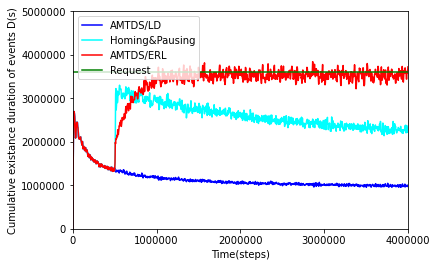
\includegraphics[width=150mm]{figures/ds_graph_3600_ave_ERL_Complex_1000.png}
    \caption{D(s)の時間推移の比較(実験6)}
    \label{fig:ds_ERL_Complex}
  \end{figure}

  \begin{figure}
    \centering
    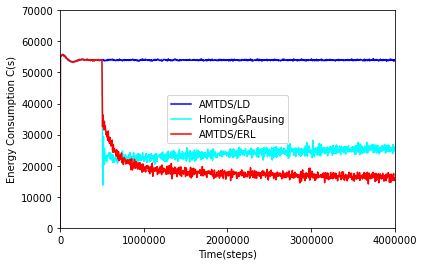
\includegraphics[width=150mm]{figures/cs_graph_3600_ave_ERL_Complex_1000.png}
    \caption{C(s)の時間推移の比較(実験6)}
    \label{fig:cs_ERL_Complex}
  \end{figure}

  \begin{figure}
    \centering
    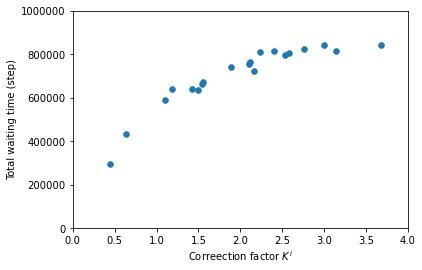
\includegraphics[width=150mm]{figures/CorrectionScatter_Complex_ERL.png}
    \caption{エージェントごとの$K^i$と総待機時間の関係(実験6)}
    \label{fig:cscatter_ERL_Complex}
  \end{figure}

  \begin{figure}
    \centering
    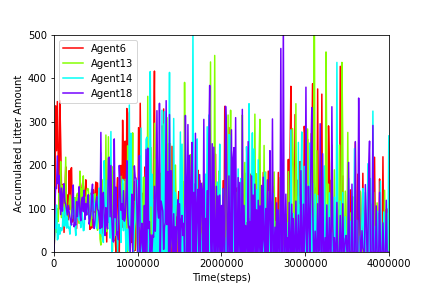
\includegraphics[width=150mm]{figures/al_graph_ERL_Complex_top.png}
    \caption{$K^i$上位4体のエージェントによるイベント処理量の時間推移(実験6)}
    \label{fig:al_ERL_Complex_top}
  \end{figure}

  \begin{figure}
    \centering
    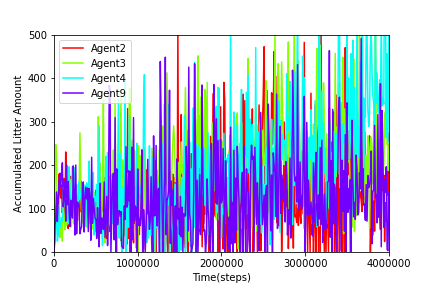
\includegraphics[width=150mm]{figures/al_graph_ERL_Complex_worst.png}
    \caption{$K^i$下位4体のエージェントによるイベント処理量の時間推移(実験6)}
    \label{fig:al_ERL_Complex_worst}
  \end{figure}

  \subsubsection{実験6: 環境の変化による性能の違い}
  \label{ex:ERL2}  
  本実験では,\ref{ex:ER2}と同様に,図\ref{fig:env2}の環境で実験を行った.
  また,比較を容易にするために,\ref{ex:ERL1}と同様に,本実験での総ステップ数は4,000,000ステップであり,要求値$D_{req}$は1,000,補正係数$K^i$の初期値は0.5である.

  \par
  まず,提案手法であるAMTDS/ERLは,異なる環境においても,D(s)の値を従来手法であるAMTDS/LDよりも増加させ,$D_{req}$に近づけ,C(s)の値をAMTDSよりも減少させることができた.
  具体的には,D(s)を$D_{req}$に近づけて約179.9\%増加させることにより,C(s)を約58.1\%削減した.
  つまり,AMTDS/ERのエネルギー節約行動により,環境全体の汚れを$D_{req}$付近にしつつ,より省エネな巡回が行うことができた.
  また,\ref{ex:ERL1}と比べると,環境全体のイベント発生量は小さくても要求値$D_{req}$を同じであるので,D(s)の増加率が大きくなるため,それに伴いC(s)の減少率も大きくなった.
  
  \par
  次に,環境全体ではなく,エージェントごとについて見ていく.
  エージェントごとの$K^i$とPausingによる総待機時間をまとめたものが表\ref{tb:ERL_Complex_k1},\ref{tb:ERL_Complex_k2},\ref{tb:ERL_Complex_k3}であり,これを散布図にまとめたものが図\ref{fig:cscatter_ERL_Complex}である.
  なお,\ref{ex:ERL1}と同様に,$K^i$は4,000,000ステップ時点の値で,総待機時間は3,000,000~4,000,000ステップでの総待機時間である.
  
  これらの表から,エージェントによって$K^i$は異なり,それによって総待機時間も異なっていることがわかる.
  また,図\ref{fig:cscatter_ERL_Office}と比較すると,全体的に充電基地での待機時間が大きくなっていることが分かる.
  これは,本実験の環境である図\ref{fig:env2}は図\ref{fig:env}と比べて環境全体のイベント発生確率が小さいため,同じ要求値$D_{req}$が与えられると,D(s)要求値付近にするためには,巡回を行わずに充電基地で待機する時間を長くしなければいけないが,待機するエージェントと待機しないエージェントという役割分担はされていないので,全体的に待機時間が増加したと考えられる.
  
  \par
  さらに,各エージェントのイベント処理量の時間推移のうち,$K^i$が上位4体を図\ref{fig:al_ER_Complex_top},下位4体を図\ref{fig:al_ER_Complex_worst}に示す.
  まず,図\ref{fig:al_ER_Complex_top}より,時間が経つにつれて$K^i$が大きくなったエージェントは,それに伴って充電基地での待機時間が長くなるため,環境を巡回する時間が短くなり,イベント処理量がだんだんと少なくなっていくことが分かる.
  逆に,図\ref{fig:al_ER_Complex_worst}より,$K^i$が小さいエージェントは,充電基地で待機することもあるのでイベント処理量が0の時もあるが,だんだんとイベント処理量が多くなっていることが分かる.
  これは,複数のエージェントの充電基地での待機時間が長くなると,ノード$v$が任意のエージェントに訪問される間隔が長くなり,それによってイベントが溜まっていくので,$K^i$が小さいエージェントのイベント処理量がだんだん多くなっていると考えられる.

  \par
  以上のことから,AMTDS/ERLは,環境が異なっても,充電基地での待機時間を変化させることによってイベント量を要求値付近にして,エネルギーを節約しながら巡回することができる手法といえる.

  \begin{table}
    \centering
    \caption{エージェント0~6における$K^i$と総待機時間の比較(実験6)}
    \begin{tabular}{lcccccccr}\\ \hline
      エージェント & 0 & 1 & 2 & 3 & 4 & 5 & 6 \\ \hline
      $K^i$ & 2.1088 & 2.3994 & 1.1821 & 0.6392 & 0.4433 & 1.4969 & 2.7605 \\ \hline
      総待機時間 & 752,000 & 815,300 & 639,100 & 430,300 & 294,800 & 636,900 & 824,800 \\ \hline
    \end{tabular}
    \label{tb:ERL_Complex_k1}
  \end{table}

  \begin{table}
    \centering
    \caption{エージェント7~13における$K^i$と総待機時間の比較(実験6)}
    \begin{tabular}{lcccccccr}\\ \hline
      エージェント & 7 & 8 & 9 & 10 & 11 & 12 & 13 \\ \hline
      $K^i$  & 1.8867 & 2.5781 & 1.0963 & 2.1660 & 2.5299 & 2.2422 & 3.1407 \\ \hline
      総待機時間 & 738,600 & 806,500 & 589,200 & 723,400 & 796,800 & 809,500 & 813,600 \\ \hline 
    \end{tabular}
    \label{tb:ERL_Complex_k2}
  \end{table}

  \begin{table}
    \centering
    \caption{エージェント14~19における$K^i$と総待機時間の比較(実験6)}
    \begin{tabular}{lccccccr}\\ \hline
      エージェント & 14 & 15 & 16 & 17 & 18 & 19 \\ \hline
      $K^i$  & 2.9975 & 2.1116 & 1.5375 &1.4290 & 3.6800 & 1.5534 \\ \hline
      総待機時間 & 841,600 & 763,000 & 660,400 & 637,800 & 839,700 & 669,600 \\ \hline
    \end{tabular}
    \label{tb:ERL_Complex_k3}
  \end{table}

  \subsubsection{実験7: エージェント数減少による性能の変化}

  \subsubsection{実験8: $K^i$の降順にエージェント数を減少させたときの性能の変化}

  \section{結論}

  \clearpage
  \bibliographystyle{junsrt}
  \bibliography{ref}

\end{document}